\documentclass[10pt]{beamer} %slightly bigger font
\usetheme{default} 
\setbeamertemplate{navigation symbols}{} %gets rid of navigation symbols
%\setbeamertemplate{footline}{} %gets rid of bottom navigation bars
%\setbeamertemplate{footline}[page number]{} %use this, if you want page numbers
%
\setbeamertemplate{itemize items}[circle] %I like round bullet points
%
\addtobeamertemplate{navigation symbols}{}{%
    \usebeamerfont{footline}%
    \usebeamercolor[fg]{title}%
    \hspace{5em}%
    \normalsize\insertframenumber/\inserttotalframenumber
}

\setlength\parskip{10pt} % I like white space between paragraphs

\setbeamertemplate{frametitle continuation}[from second][ ]

% Here is a `helper' functions to save typing, later
\newcommand{\mystart}[1]{ \section{#1}\begin{frame}[allowframebreaks, fragile] \frametitle{#1} } 

%\usepackage{float}
%\usepackage{bbm}
%\usepackage{amsmath}
%\usepackage{amssymb}
%\usepackage{ulem}
%\usepackage{subfig}
%\usepackage{sidecap}
%\usepackage{wrapfig}
%\usepackage{url}
%


\usepackage{graphicx}
\usepackage{wrapfig}
\usepackage{subfig}
\usepackage{sidecap}
\usepackage{fancyvrb}
\usepackage{algorithm}
\usepackage{algorithmic}



\newcommand{\xmark}{\ding{55}}%
\newcommand{\Ell}{\mathcal{L}}
\newcommand{\mb}{\mathbf}
\newcommand{\indfun}[1]{\ensuremath{\mb{1}_{\{#1\}}}}
\newcommand{\E}{\mathbbm{E}}
\DeclareMathOperator*{\argmin}{argmin}

\newcommand{\ind}{\mathbbm{1}}
\newcommand{\R}{\mathbb{R}}
\newcommand{\C}{\mathbb{C}}
\newcommand{\Z}{\mathbb{Z}}

\fvset{frame=none,framesep=0mm,fontsize=\tiny,numbers=none,framerule=0mm,numbersep=1mm,commandchars=\\\{\}}

%\mode<presentation>
%{
%  \usetheme{Boadilla}      % or try Darmstadt, Madrid, Warsaw, ...
%  \usecolortheme{beaver} % or try albatross, beaver, crane, ...
%  \usefonttheme{default}  % or try serif, structurebold, ...
%  \setbeamertemplate{navigation symbols}{}
%  \setbeamertemplate{caption}[numbered]
%
%
%}


%\usepackage{media9}
\usepackage{animate}

%% For \subfloat command
\usepackage{subfig}

\usepackage{color}
\newcommand{\blue}[1]{{\color{blue} #1} }
\newcommand{\red}[1]{{\color{red} #1} }
\definecolor{mygray}{rgb}{0.95,0.95,0.95}
\newcommand{\myGray}[1]{{\color{mygray} #1} }
\usepackage{tikz,pgfpages}
\usepackage{amsmath,amssymb}
\usetikzlibrary{shapes,arrows,trees,mindmap,decorations.pathreplacing}

\usepackage{algorithm,algorithmic}

\usepackage{cancel}

%\newcommand{\amp}{\mathop{\:\:\,}\nolimits}
%
%\newcommand{\prox}{\mathop{\rm prox}\nolimits}

\newtheorem{proposition}{Proposition}
%\newtheorem{example}{Example}
%\newtheorem{definition}{Definition}
\newcommand{\svskip}{\vspace{1.75mm}}
\def\E{\mathop{\rm E\,\!}\nolimits}
\def\Var{\mathop{\rm Var}\nolimits}
\def\Cov{\mathop{\rm Cov}\nolimits}
\def\trace{\mathop{\rm trace}\nolimits}
\def\logdet{\mathop{\rm \logdet}\nolimits}
\def\vec{\mathop{\rm vec}\nolimits}
\def\den{\mathop{\rm den}\nolimits}
\def\midd{\mathop{\,|\,}\nolimits}
\def\sgn{\mathop{\rm sgn}\nolimits}
\def\sinc{\mathop{\rm sinc}\nolimits}
\def\curl{\mathop{\rm curl}\nolimits}
\def\div{\mathop{\rm div}\nolimits}
\def\tr{\mathop{\rm tr}\nolimits}
\def\len{\mathop{\rm len}\nolimits}
\def\cond{\mathop{\rm cond}\nolimits}
\def\conv{\mathop{\rm conv}\nolimits}
\def\dom{\mathop{\rm dom}\nolimits}
\def\epi{\mathop{\rm epi}\nolimits}
\def\graph{\mathop{\rm graph}\nolimits}
\def\cl{\mathop{\rm cl}\nolimits}
\def\diag{\mathop{\rm diag}\nolimits}
\def\dist{\mathop{\rm dist}\nolimits}
\def\prox{\mathop{\rm prox}\nolimits}
\def\argmin{\mathop{\rm argmin}\nolimits}
\def\gph{\mathop{\rm gph}\nolimits}
\def\amp{\mathop{\;\:}\nolimits}
\newcommand{\ba}{\boldsymbol{a}}
\newcommand{\bb}{\boldsymbol{b}}
\newcommand{\bc}{\boldsymbol{c}}
\newcommand{\bd}{\boldsymbol{d}}
\newcommand{\be}{\boldsymbol{e}}
\newcommand{\bff}{\boldsymbol{f}}
\newcommand{\bg}{\boldsymbol{g}}
\newcommand{\bh}{\boldsymbol{h}}
\newcommand{\bi}{\boldsymbol{i}}
\newcommand{\bj}{\boldsymbol{j}}
\newcommand{\bk}{\boldsymbol{k}}
\newcommand{\bl}{\boldsymbol{l}}
\newcommand{\bm}{\boldsymbol{m}}
\newcommand{\bn}{\boldsymbol{n}}
\newcommand{\bo}{\boldsymbol{o}}
\newcommand{\bp}{\boldsymbol{p}}
\newcommand{\bq}{\boldsymbol{q}}
\newcommand{\br}{\boldsymbol{r}}
\newcommand{\bs}{\boldsymbol{s}}
\newcommand{\bt}{\boldsymbol{t}}
\newcommand{\bu}{\boldsymbol{u}}
\newcommand{\bv}{\boldsymbol{v}}
\newcommand{\bw}{\boldsymbol{w}}
\newcommand{\bx}{\boldsymbol{x}}
\newcommand{\by}{\boldsymbol{y}}
\newcommand{\bz}{\boldsymbol{z}}
\newcommand{\bA}{\boldsymbol{A}}
\newcommand{\bB}{\boldsymbol{B}}
\newcommand{\bC}{\boldsymbol{C}}
\newcommand{\bD}{\boldsymbol{D}}
\newcommand{\bE}{\boldsymbol{E}}
\newcommand{\bF}{\boldsymbol{F}}
\newcommand{\bG}{\boldsymbol{G}}
\newcommand{\bH}{\boldsymbol{H}}
\newcommand{\bI}{\boldsymbol{I}}
\newcommand{\bJ}{\boldsymbol{J}}
\newcommand{\bK}{\boldsymbol{K}}
\newcommand{\bL}{\boldsymbol{L}}
\newcommand{\bM}{\boldsymbol{M}}
\newcommand{\bN}{\boldsymbol{N}}
\newcommand{\bO}{\boldsymbol{O}}
\newcommand{\bP}{\boldsymbol{P}}
\newcommand{\bQ}{\boldsymbol{Q}}
\newcommand{\bR}{\boldsymbol{R}}
\newcommand{\bS}{\boldsymbol{S}}
\newcommand{\bT}{\boldsymbol{T}}
\newcommand{\bU}{\boldsymbol{U}}
\newcommand{\bV}{\boldsymbol{V}}
\newcommand{\bW}{\boldsymbol{W}}
\newcommand{\bX}{\boldsymbol{X}}
\newcommand{\bY}{\boldsymbol{Y}}
\newcommand{\bZ}{\boldsymbol{Z}}
\newcommand{\balpha}{\boldsymbol{\alpha}}
\newcommand{\bbeta}{\boldsymbol{\beta}}
\newcommand{\bgamma}{\boldsymbol{\gamma}}
\newcommand{\bdelta}{\boldsymbol{\delta}}
\newcommand{\bepsilon}{\boldsymbol{\epsilon}}
\newcommand{\blambda}{\boldsymbol{\lambda}}
\newcommand{\bmu}{\boldsymbol{\mu}}
\newcommand{\bnu}{\boldsymbol{\nu}}
\newcommand{\bphi}{\boldsymbol{\phi}}
\newcommand{\bpi}{\boldsymbol{\pi}}
\newcommand{\bsigma}{\boldsymbol{\sigma}}
\newcommand{\btheta}{\boldsymbol{\theta}}
\newcommand{\bzeta}{\boldsymbol{\zeta}}
\newcommand{\bomega}{\boldsymbol{\omega}}
\newcommand{\bGamma}{\boldsymbol{\Gamma}}
\newcommand{\bDelta}{\boldsymbol{\Delta}}
\newcommand{\bTheta}{\boldsymbol{\Theta}}
\newcommand{\bLambda}{\boldsymbol{\Lambda}}
\newcommand{\bXi}{\boldsymbol{\Xi}}
\newcommand{\bPi}{\boldsymbol{\Pi}}
\newcommand{\bSigma}{\boldsymbol{\Sigma}}
\newcommand{\bUpsilon}{\boldsymbol{\Upsilon}}
\newcommand{\bPhi}{\boldsymbol{\Phi}}
\newcommand{\bPsi}{\boldsymbol{\Psi}}
\newcommand{\bOmega}{\boldsymbol{\Omega}}

\newcommand{\source}[1]{\caption*{Source: {#1}} }



\title[]{Scalable algorithms for GWAS, genotype imputation, and ancestry inference}
\author[Benjamin Chu]{Benjamin Chu}
\institute[UCLA]{Graduate program in Biomathematics\\
Department of Computational Medicine\\
University of California, Los Angeles}

\date{Stanford (online), December 10, 2020}

%\epstopdfDeclareGraphicsRule{.gif}{png}{.png}{convert gif:#1 png:\OutputFile}
%\AppendGraphicsExtensions{.gif}

\AtBeginSection[]
{
 \begin{frame}<beamer>
 \frametitle{Outline}
 \tableofcontents[currentsection]
 \end{frame}
}
\includeonly{struct}

\setbeamercovered{transparent}
\begin{document}
\frame{\titlepage}

\frame{
\frametitle{Outline}
\begin{itemize}
    \item Phasing, Imputation, and admixture estimation
    \begin{itemize}
        \item Introduction
        \item What we did
        \item Potential future projects
    \end{itemize}
    \item IHT for association studies
    \begin{itemize}
        \item Introduction
        \item What we did
        \item Potential future projects
    \end{itemize}
\end{itemize}
}

\begin{frame}{}
  \centering \Large
  Part 1: Imputation, phasing, and admixture inference
\end{frame}

\frame{
\frametitle{What is genotype imputation?}
\begin{itemize}
    \item Michigan Imputation Server imputes $>10$ million genomes annually
    \item Purpose: increase number of markers; meta analysis
    \item Inputs
    \begin{enumerate}
        \item GWAS data with $\sim 10^6$ unphased genotypes (entries $0, 1, 2$)
        \item Reference panel with $10^7\sim10^8$ phased genotypes (entries $0, 1$) 
    \end{enumerate}
    \item Output: Phased genotypes at all markers
\end{itemize}
\begin{figure}
    \centering
    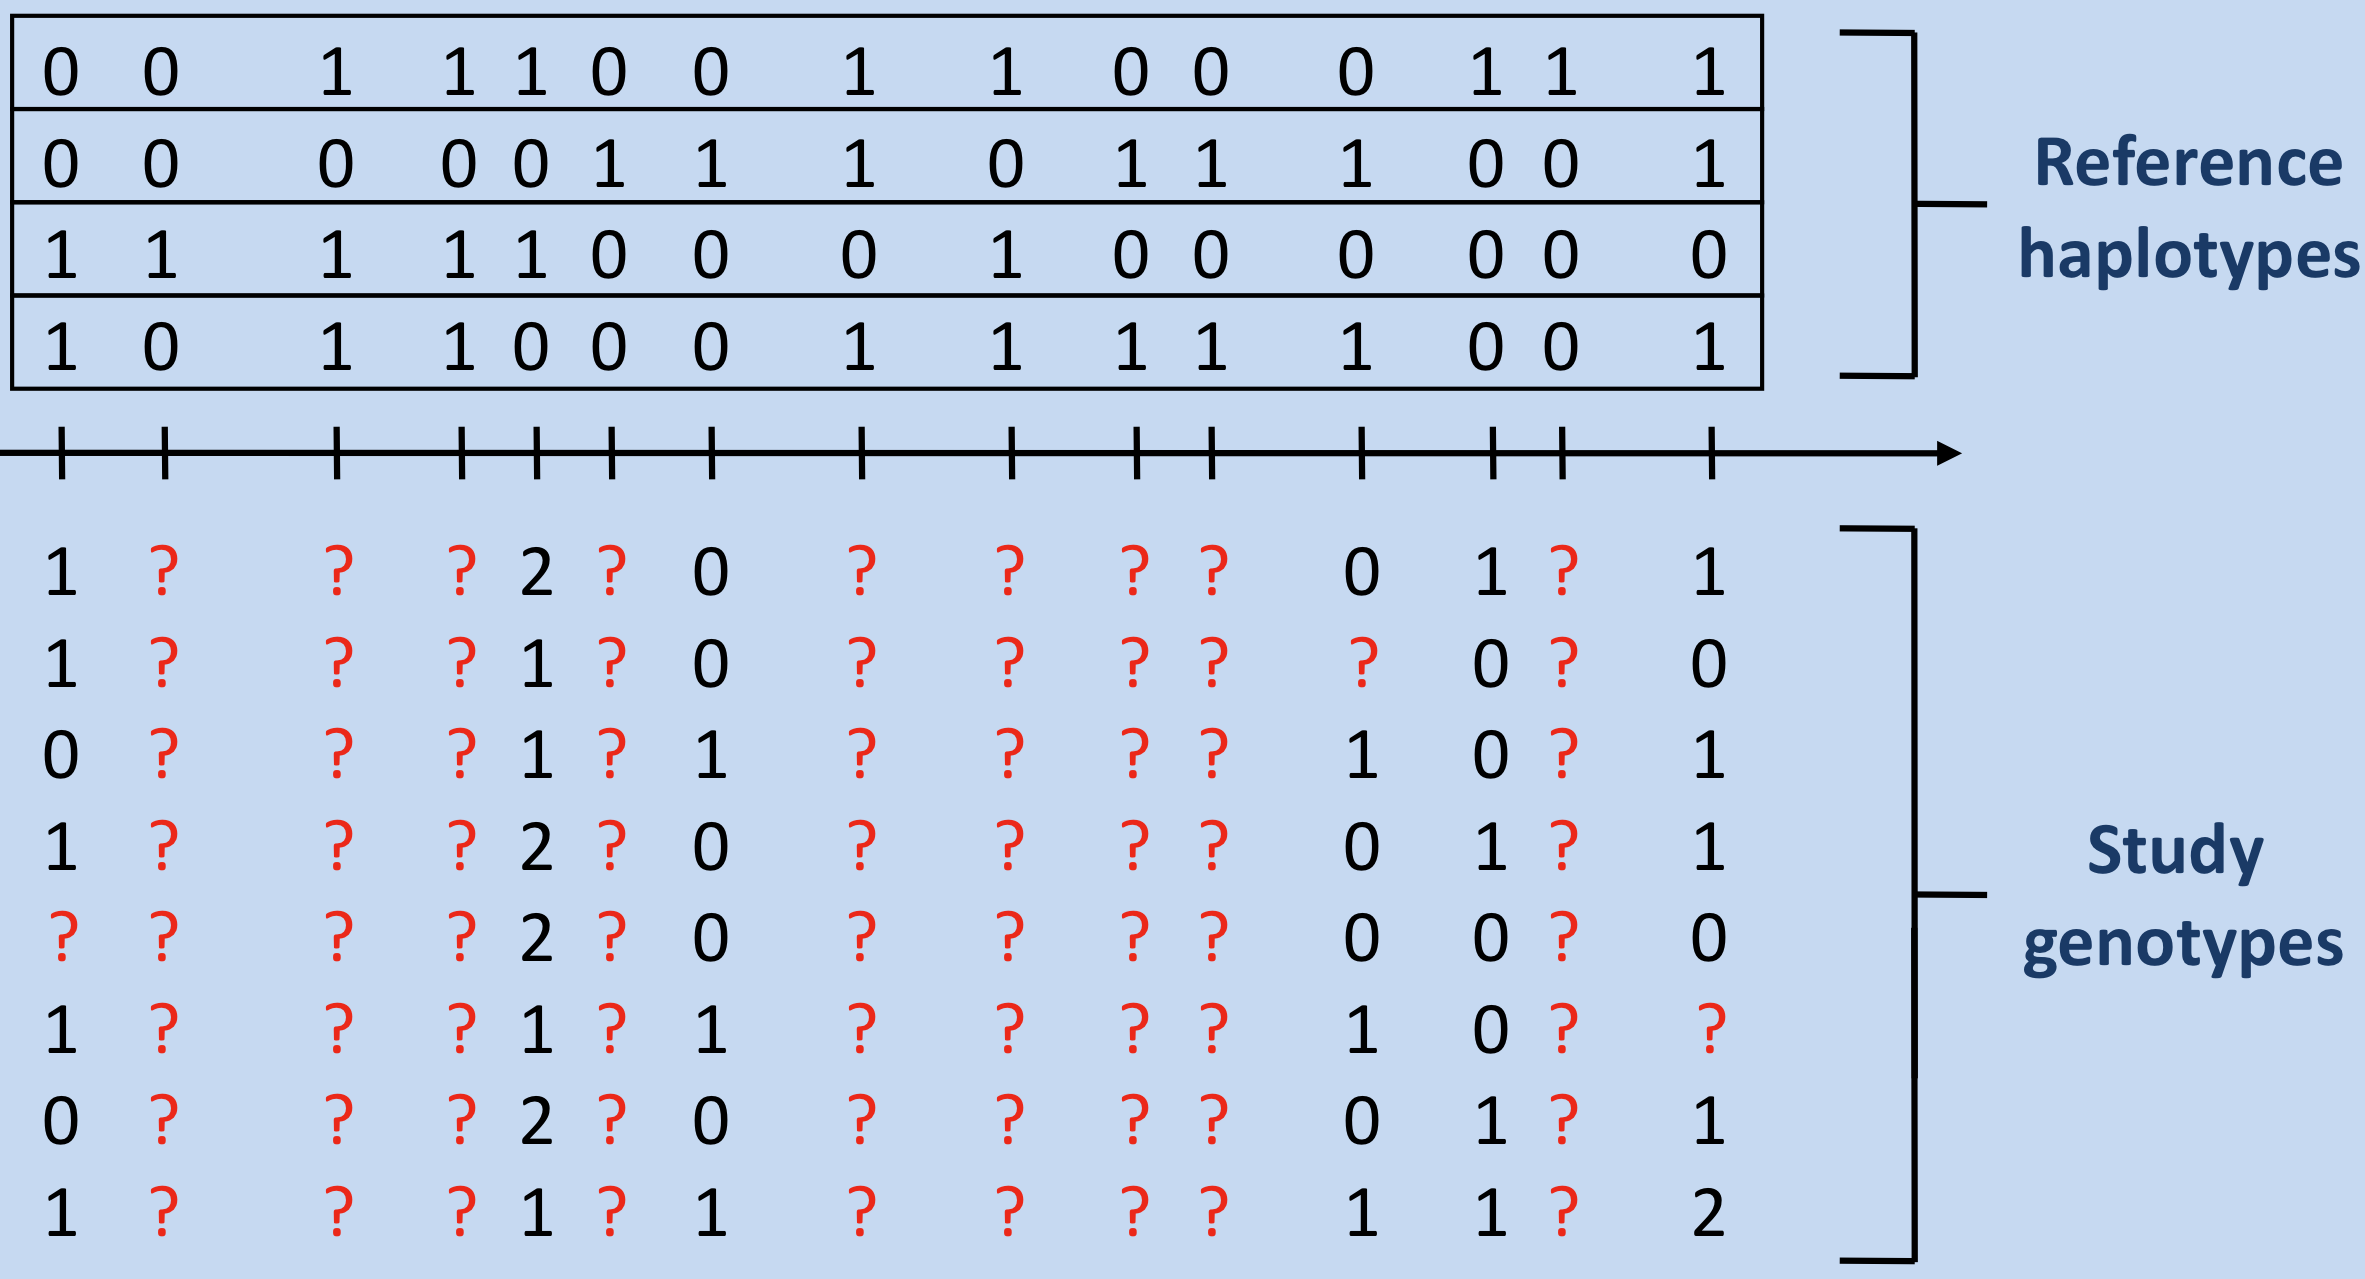
\includegraphics[width=3in]{figures/imputation.png}
    \source{\small\url{http://mathgen.stats.ox.ac.uk/impute/impute_v2.html}}
\end{figure}
}

\frame{
\frametitle{Background}
\begin{itemize}
    \item Reference panels are getting \textbf{big}!
    \begin{itemize}
        \item 2012: 1k samples at 28M SNPs (1000 genomes phase 1)
        \item 2016: 32k samples at 39M SNPs (Haplotype reference consortium)
        \item 2019: 97k samples at 308M sites from sequences (TOPMed)
    \end{itemize}
    \item Genotype imputation usually employ hidden Markov models (HMM)
    \begin{itemize}
        \item e.g. Minimac 4, Beagle 5.1, Impute 5
        \item All based on Li and Stephens, {\it Genetics, 165(4):2213–2233, 2003} 
        \item Very similar accuracy
        \item Requires prephasing data = chaining softwares
    \end{itemize}
    \item HMM methods are slow!
    \begin{itemize}
        \item They are $>10,000$ times faster since version 1 of the initial software, but some problems are still (increasingly) unmanageable. 
    \end{itemize}
\end{itemize}
}

\frame{
\frametitle{Case study: HMM methods are slow}
Using Minimac 4 (used on imputation server),
    \begin{itemize}
        \item Imputing 1000 samples\footnote{on local computer: 64 GB RAM; Intel i9 9920X CPU with 12 cores}, with HRC panel (2016) requires $12,892$ seconds $\approx$ \alert{3.5h} on chromosome 10
        \item With 23 pairs chromosome and 500k samples in UK Biobank, this imputation will take $3.5 \times 23 \times 500$ hours $\approx $ \alert{\textbf{4.7}} years.
    \end{itemize}
    
    Our software \texttt{MendelImpute.jl} \begin{itemize}
        \item takes $\sim$ 20 days
        \item requires no prephasing and much less computer memory
        \item generates ancestry data automatically
        \item might lead to better data compression
    \end{itemize}
}

\frame{
\frametitle{Imputation within a small genomic region (window)}
Consider genotype vector $\bx$ and (unique) reference haplotypes $\bh_1, ..., \bh_d$ in the small genomic window. Imputation is done by minimizing
\begin{align*}
    ||\bx - \bh_i - \bh_j||_2^2 = ||\bx||^2_2 + ||\bh_i||^2_2 + ||\bh_j||^2_2 + 2\bh_i^t\bh_j - 2\bx^t\bh_i - 2\bx^t\bh_j
\end{align*}
over all $\bh_i, \bh_j$ pairs. Solution:
\begin{enumerate}
    \item Collect $||\bh_i||^2_2 + ||\bh_j||^2_2+2\bh_i^t\bh_j$ terms into matrix $\bM$
    \item Collect $-2\bx^t\bh_i - 2\bx^t\bh_j$ terms into matrix $\bN$
    \item Search for the minimum in the upper triangular matrix $\bM + \bN$
\end{enumerate}
where
\begin{itemize}
    \item $\bM, \bN$ are efficiently assembled from $\bH^t\bH$ and $\bX^t\bH$
    \item Parallelization is achieved by treating different windows independently
\end{itemize}
}

\frame{
\frametitle{Phasing: extend haplotypes across windows}
\begin{itemize}
    \item Unique haplotypes $\bh_i, \bh_j$ expands to sets of equivalent haplotypes. 
    \item These sets are intersected across windows.
    \item Eventually intersection becomes empty, representing ancient or contemporary recombination events
    \item We parallelize phasing over samples, since samples are independent.
\end{itemize}
\begin{figure}
    \centering
    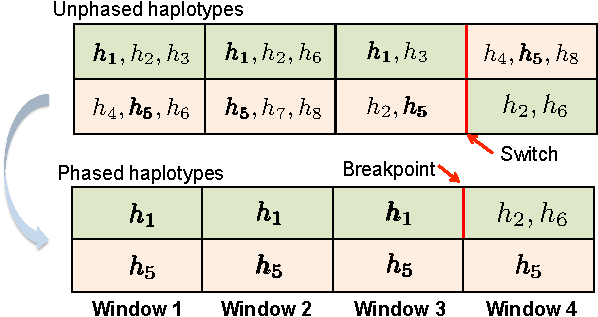
\includegraphics[width=10cm]{figures/d.pdf}
\end{figure}
}

\frame{
\frametitle{Comparison with HMM methods}
\begin{table}
\centering
\small
\begin{tabular}{l|c|c|c}
    \hline
    \hline
    \textbf{1000G chr10}  & {Error Rate} & {Time (sec)} & {Memory (GB)} \\
    \hline
    \texttt{MendelImpute} & 1.09E-02 &  39       & 3.7\\
    \texttt{Beagle} 5.1   & 5.51E-03 & 196       & 9.6\\
    \texttt{Minimac} 4    & 5.24E-03 & 728 & 10.2\\
    \hline
    \hline
    \textbf{1000G chr20}  & {Error Rate} & {Time (sec)} & {Memory (GB)} \\
    \hline
    \texttt{MendelImpute} & 3.28E-02 &  13      & 2.6\\
    \texttt{Beagle} 5.1   & 1.68E-02 &  33      & 4.9\\
    \texttt{Minimac} 4    & 1.65E-02 & 159 & 5.0\\
    \hline
    \hline
    \textbf{HRC chr10}    & {Error Rate} & {Time (sec)} & {Memory (GB)} \\
    \hline
    \texttt{MendelImpute} & 6.87E-03 &   154        &  7.3\\
    \texttt{Beagle} 5.1   & 1.90E-03 &  1961        & 32.4\\
    \texttt{Minimac} 4    & 1.71E-03 & 14604 & 22.5\\
    \hline
    \hline
    \textbf{HRC chr20}    & {Error Rate} & {Time (sec)} & {Memory (GB)} \\
    \hline
    \texttt{MendelImpute} & 1.36E-03 &   133        &  6.2\\
    \texttt{Beagle} 5.1   & 5.28E-04 &  2457        & 27.4\\
    \texttt{Minimac} 4    & 6.34E-04 & 17507 & 33.2\\ 
    \hline
    \hline
\end{tabular}
\end{table}
Conclusion: 10-100x faster, 3-5x more memory efficient, 2-4x less accurate. 
}

\frame{
\frametitle{Extension to ancestry inference}
\begin{itemize}
    \item After imputation, each (unphased)  genotype is decomposed into a mosaic of haplotype segments from the reference panel.
    \item If reference samples are labeled with ethnic or country origin, we can visualize local ancestry pattern. We call this \alert{chromosome painting}.
\end{itemize}
\begin{figure}
    \centering
    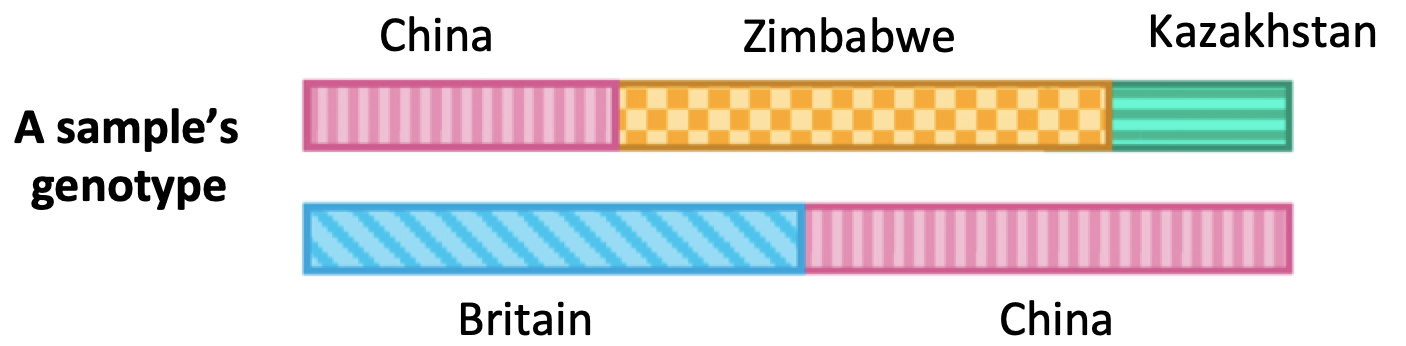
\includegraphics[width=4in]{figures/chrompaint_illustration.png}
\end{figure}
}


\frame{
\frametitle{Test data: 1000 genomes project (v3)}
\begin{itemize}
    \item 2504 samples from 26 populations
    \item Many admixed, many not (4 grandparents all from local area)
    \item Does not include Native American populations
\end{itemize}
\begin{figure}
    \centering
    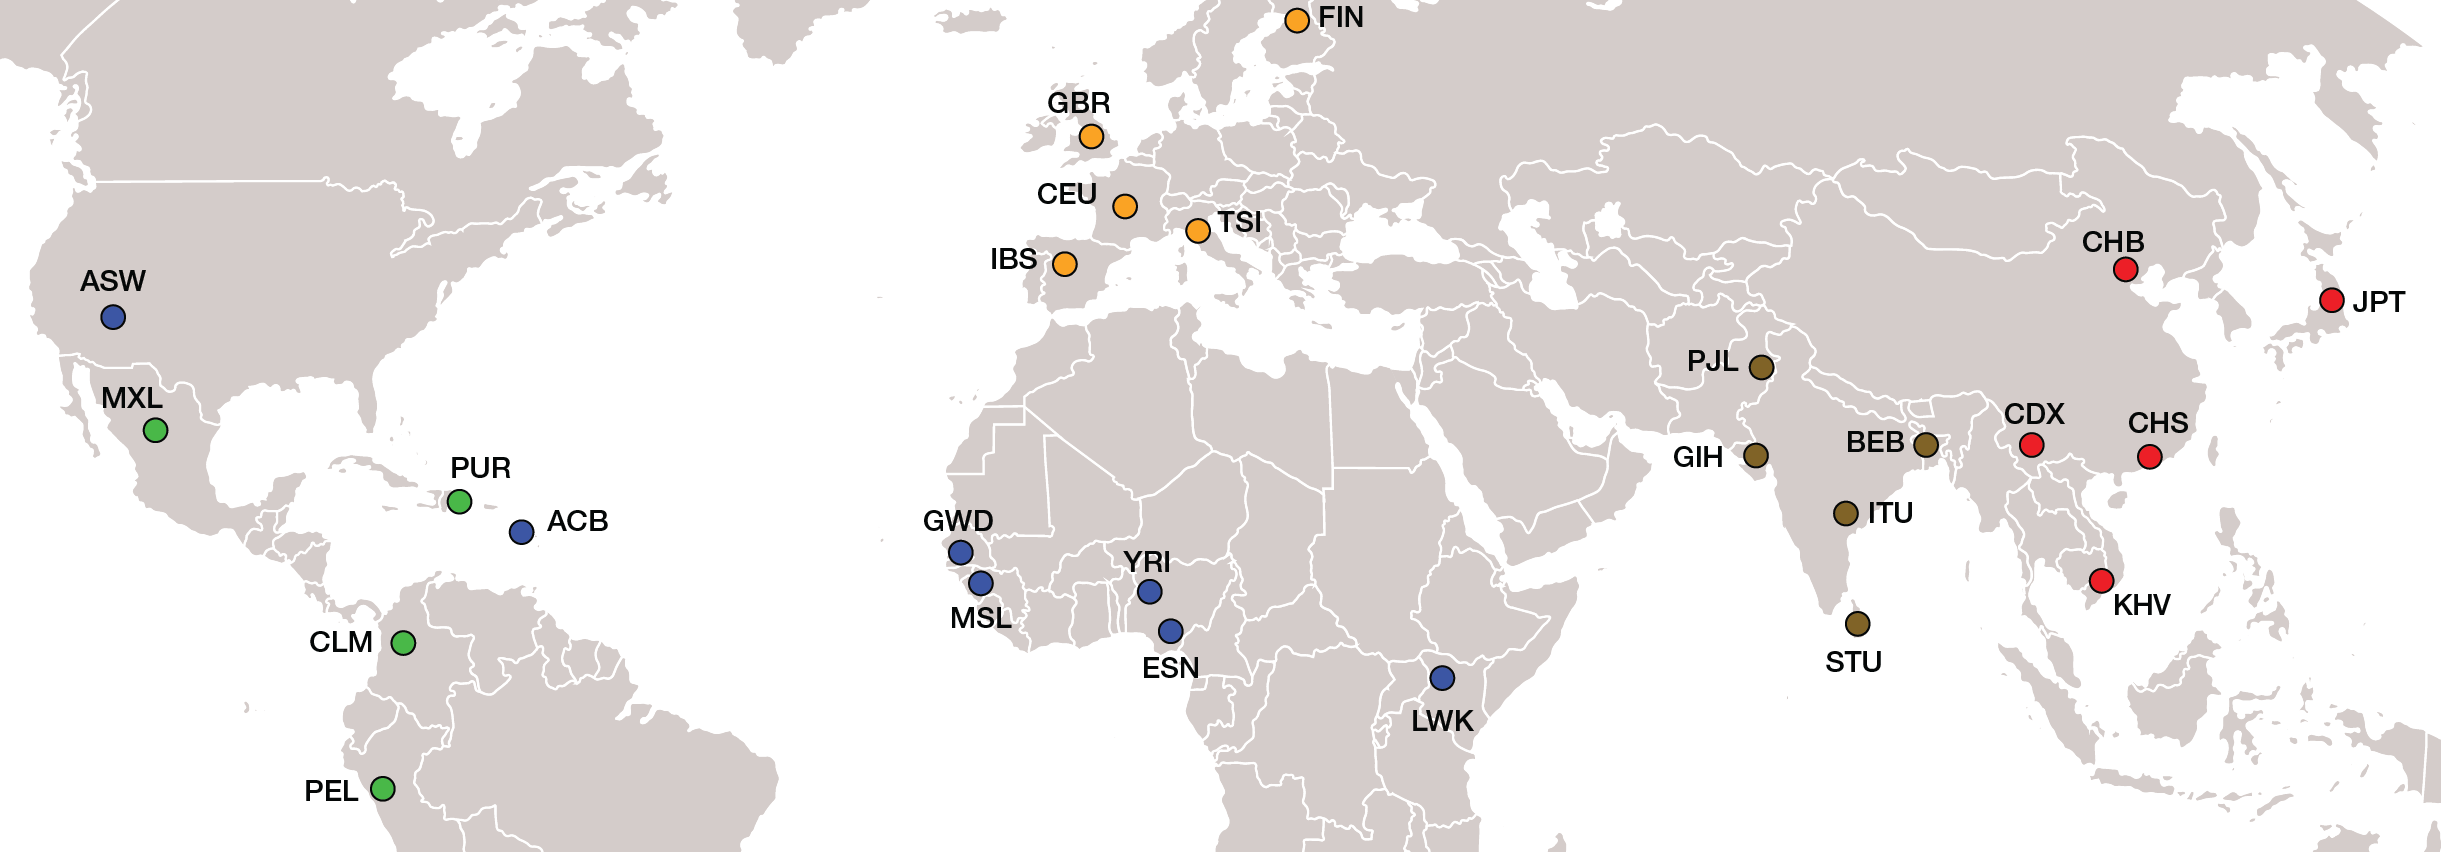
\includegraphics[width=11cm]{figures/1000gp_popMap.png}
    \source{https://gadget.biosci.gatech.edu/learn.html}
\end{figure}
}

\frame{
\frametitle{Chromosome 18 painting on PUR, PEL, and ASW}
\begin{figure}
    \centering
    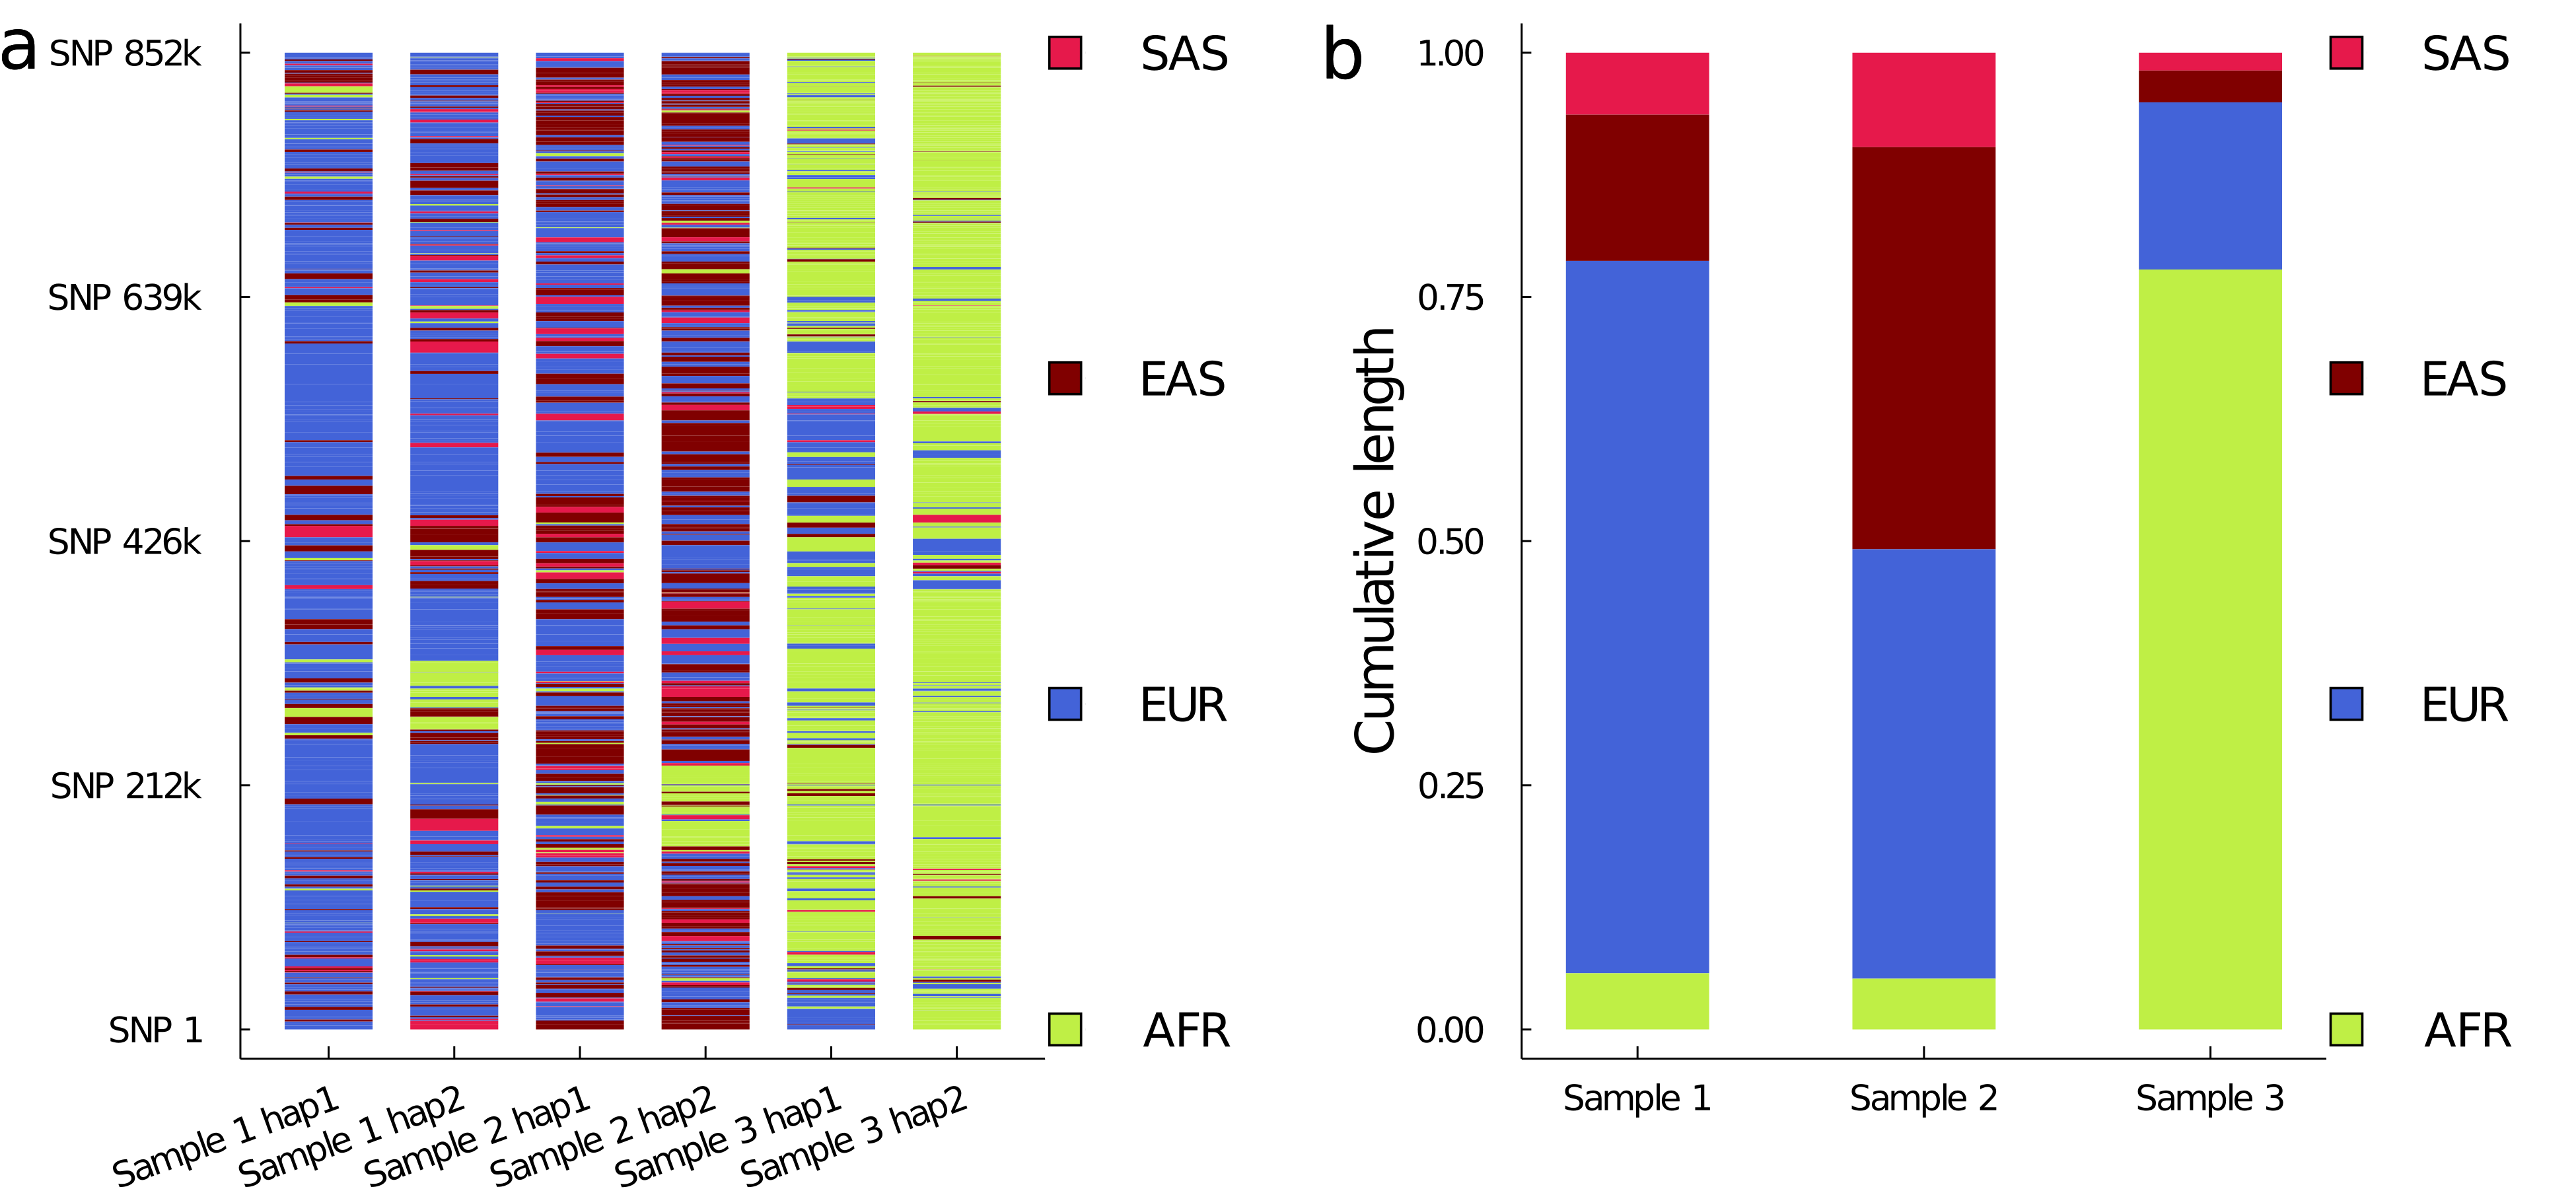
\includegraphics[height=2in]{figures/admixture_superpopulation.png}
\end{figure}
For comparison, their ADMIXTURE estimates are
\begin{itemize}
    \item PUR (Peurto Rican): 0.164589, 0.136001, 0.647827, 0.051582
    \item PEL (Peruvian): 0.803278, 0.175677, 1.0e-5, 0.021035
    \item ASW (African American): 1.0e-5, 0.140135, 1.0e-5, 0.859845
\end{itemize}
}

\frame{
\frametitle{Data Compression}
\begin{itemize}
    \item Large genotype files are painful to transfer. 
    \item Data compression can be achieved by phasing. Simply send:
    \begin{enumerate}
        \item Start position for each haplotype segment
        \item Pointer to the relevant haplotype in the reference panel
    \end{enumerate}
\end{itemize}

\begin{table}
\centering
\begin{tabular}{|l|c|c|c|}
    \hline
    Data Set    &   {vcf.gz}  & {compressed} & {compression} \\
                & {size (MB)} &    {size (MB)}     &   {ratio}     \\
    \hline
    Sim 10K     &  10.07 & 0.05 & 201\\
    Sim 100K    &  10.71 & 0.04 & 267\\
    Sim 1M      &  11.05 & 0.04 & 276\\
    1000G Chr10 &  31.53 & 1.37 &  23\\
    1000G Chr20 &  13.93 & 0.43 &  46\\
    HRC Chr10   & 155.71 & 7.47 &  21\\
    HRC Chr20   &  70.42 & 5.86 &  12\\
    \hline
\end{tabular}
\caption{Output file size comparison of VCF and our compression strategy.}
\end{table}
}

% \frame{
% \frametitle{Challeneges of Imputation}
% \begin{enumerate}
%     \item Need large, \textbf{ethnically diverse} samples in the reference panel
%     \item Need universally accessible reference panels stored on the cloud
% \end{enumerate}
% }

\frame{
\frametitle{Potential future work}
\begin{enumerate}
    \item Ancestry inference
    \begin{itemize}
        \item Quantify linkage patterns
        \item Promote new use for reference panels: deriving ancestry information
        \item Construct different confidence level for different haplotype segments
    \end{itemize}
    \item \texttt{MendelImpute2}: Improve error rate
    \begin{itemize}
        \item How to account for within-window breakpoints?
        \item Implement overlapping windows strategy
        \item Parallel data import
    \end{itemize}
    \item Compare output haplotypes across programs
\end{enumerate}
}

\begin{frame}{}
  \centering \Large
  Part 2: Iterative hard thresholding in Genome wide association studies
\end{frame}

\frame{
\frametitle{Genome wide association studies}
\begin{itemize}
    \item We want to study genetic basis of a (\alert{usually continuous}) phenotype
    \begin{itemize}
        \item Examples: Height, developed cancer, number of seeds per plant
    \end{itemize}
    \item Recruit $n$ samples, genotype each sample at $p$ SNPs, producing
    \begin{align*}
        \bX^{n \times p} = 
        \begin{pmatrix}
            x_{11} & \cdots & x_{1p}\\
            \vdots & & \vdots\\
            x_{n1} & \cdots & x_{np}
        \end{pmatrix}, \quad x_{ij} \in \{0, 1, 2\}
    \end{align*}
    \item Also measure each individual’s phenotype 
    \begin{align*}
        \by =
        \begin{pmatrix}
            y_1 \\
            \vdots\\
            y_n
        \end{pmatrix}
    \end{align*}
    \item Goal: which SNPs are associated with the phenotype?
\end{itemize}
}

\frame{
\frametitle{Methods for Associations Testing}
\begin{enumerate}
    \item Naive model
    \begin{itemize}
        \item $\by =  \bX\bbeta + \bepsilon, \quad \bepsilon \sim N(0, \sigma^2_e\bI)$
        \item Method: solve $\argmin_{\bbeta}||\by-\bX\bbeta||^2_2$ with solution $\hat{\bbeta} = (\bX^t\bX)^{-1}\bX\by$
        \item Comments: There are $\infty$ solutions since $p > n$
    \end{itemize}
    \item Marginal association model
    \begin{itemize}
        \item $\by = \bx_{j}\beta_j + \bepsilon, \quad \bepsilon \sim N(0, \sigma^2_e\bI)$
        \item Method: hypothesis testing for each SNP: $H_0: \beta_j = 0, H_a: \beta_j \ne 0$
        \begin{itemize}
            \item Score test, LRT, Wald test ...etc
            \item Reject $H_0$ if $p < 5 \times 10^{-8}$
        \end{itemize}
        \item Comment: Assumes every SNP is independent of each other
    \end{itemize}
    \item Linear mixed model
    \begin{itemize}
        \item $\by = \bx_{j}\beta_j + \bepsilon, \quad \bepsilon \sim N(0, \frac{\sigma_g^2}{p}\bX\bX^t + \sigma_e^2I)$
        \item Method: hypothesis testing for each SNP: $H_0: \beta_j = 0, H_a: \beta_j \ne 0$
        \item Comment: Hard to estimate $\sigma_g, \sigma_e$. Expensive to form $\bX\bX^t$. Have to calculate determinants and solve huge linear equations. \alert{Current analysis methods scale poorly for non-Gaussian phenotypes}
    \end{itemize}
    \item Penalized regression
\end{enumerate}
}

\frame{
\frametitle{Option 4: Penalized regression methods}

Minimize the original model $\ell(\bbeta) = ||\by-\bX\bbeta||^2_2$ plus constraints $p(\bbeta, \blambda)$. \\~\
\begin{itemize}
    \item {\bf lasso}: minimize $f(\bbeta) = \ell(\bbeta) + \lambda ||\bbeta||_1$
    \item {\bf MCP}: minimize $f(\bbeta) = \ell(\bbeta) + \sum_{i=2}^p q(|\beta_j|)$ where
    \begin{align*}
        q(\beta_i) =
        \begin{cases}
            \lambda\beta_i - \beta_i^2/(2\lambda) & 0 \le \beta_i \le \gamma \lambda\\
            \gamma\lambda^2/2 & \beta_i > \gamma\lambda
        \end{cases}
    \end{align*}
    \item {\bf Iterative hard thresholding (IHT):}
    \begin{align*}
        \text{minimize} \quad  \ell(\bbeta) \quad s.t. \quad ||\bbeta||_0 \le k. \quad
    \end{align*}
\end{itemize}

Shrinkage of lasso tend to encourage too many false positives. The $\ell_0$ norm of IHT enforces sparsity without shrinkage.

% \begin{figure}
%     \centering
%     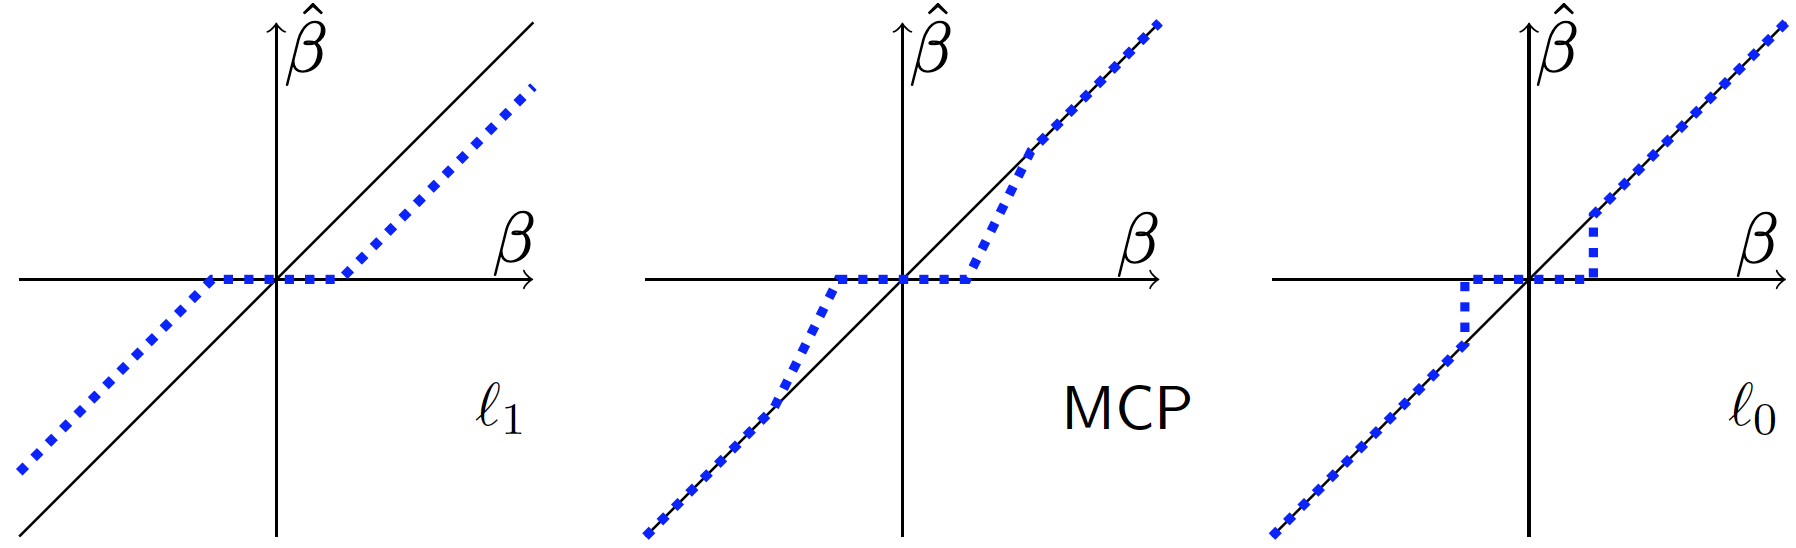
\includegraphics[width=3in]{figures/shrinkage2.png}
% \end{figure}
}

\frame{
\frametitle{IHT background}
\textbf{Problem}: minimizes $f(\bbeta) = ||\by-\bX\bbeta||^2_2 \quad s.t. \quad ||\bbeta||_0 \le k \in \Z.$\\~\

\textbf{Solution: } IHT iterates via
\begin{align*}
    \bbeta_{n+1} = \overbrace{P_{S_k}}^{(3)}\big(\bbeta_n - \underbrace{s_n}_{(2)} \overbrace{\nabla f(\bbeta_n)}^{(1)}\big).
\end{align*}

\begin{enumerate}
    \item Compute gradient $\nabla f(\bbeta) = -\bX^t(\by - \bX\bbeta)$
    \item Compute step size $s = \frac{||\nabla f(\bbeta)||^2}{\nabla f(\bbeta)^tJ(\bbeta)\nabla f(\bbeta)} > 0$
    \item Project to sparsity by setting all but $k$ largest entries to $0$. 
\end{enumerate}
}

% \frame{
% \frametitle{Choosing step size $s_n$}
% If the support does not change at iteration $n+1$, IHT's iteration simplifies to  $\bbeta_{n+1} = \bbeta_n + s_n\bv_n$ where $\bv_n = -\nabla f(\bbeta_n)$. Thus \begin{align*}
%     f(\bbeta_{n+1}) &= f(\bbeta_{n} + s_n\bv_n) 
%     = f(\bbeta_{n}) + s_n\nabla f(\bbeta_n)^t\bv_n + \frac{s_n^2}{2}\bv_n^td^2f(\bbeta_n)\bv_n\\
%     &= f(\bbeta_n) - s_n||\nabla f(\bbeta_n)^t|| + \frac{s_n^2}{2}\nabla f(\bbeta_n)^t d^2f(\bbeta_n) \nabla f(\bbeta_n)
% \end{align*}
% Differentiate w/r to $s_n$ and setting to zero, the min occurs at
% \begin{align*}
%     \boxed{s_n = \frac{||\nabla f(\bbeta_n)||_2^2}{\nabla f(\bbeta_n)^t d^2f(\bbeta_n) \nabla f(\bbeta_n)}}
% \end{align*}
% where $d^2f(\bbeta_n) = \nabla \left[-\bX^t(\by - \bX\bbeta)\right] = \bX^t\bX$.
% }

\frame{
\frametitle{Generalized linear models for non-Gaussian phenotypes}
For \alert{non-Gaussian} phenotypes (e.g. $y_i \in \{0, 1\}$) we can model $y_i$ as generalized linear models (GLM)
\begin{align*}
    \mu_i = \E(y_i) = g(\bx_i^t\bbeta)
\end{align*}
where $g$ is a nonlinear inverse link function. The loglikelihood, score (gradient), and expected information (expected negative Hessian) is
\begin{align*}
    L(\bbeta) &= \sum_{i=1}^n \left[\frac{y_i\theta_i - b(\theta_i)}{a(\phi_i)}+c(y_i, \phi_i)\right] \approx \sum_{i=1}^n \left[ \frac{y_ig(\bx_i^t\bbeta) - b[g(\bx_i^t\bbeta)]}{a(\phi_i)} \right]\\
    \nabla L(\bbeta) &= \sum_{i=1}^n(y_i - \mu_i)\frac{b''[g(\bx_i^t\bbeta)]g'(\bx_i^t\bbeta)}{\sigma_i^2}\bx_i^t = \bX^t\bW_1(\by - \bmu)\\
    J(\bbeta) &= \sum_{i=1}^n \frac{b''[g(\bx_i^t\bbeta)]^2}{\sigma_i^2}g'(\bx_i^t\bbeta)\bx_i\bx_i^t = \bX^t\bW_2\bX
\end{align*}
where $y_i$ has mean $\mu_i = b'[g(\bx_i^t\bbeta)]$ and variance $\sigma_i^2 = b''[g(\bx_i^t\bbeta)]a(\phi_i)$. \alert{These provide all the necessary ingredients for running IHT on GLMs.} 
}

\frame{
\frametitle{We also did a few more things...}
\begin{itemize}
    \item Derivation for optimal step size $s_n$ for each IHT iteration 
    \item Doubly sparse projection for sparsity within and between groups.
    \item Incorporation of prior weights.
    \item Block estimation for nuisance parameters
\end{itemize}
}

% \frame{
% \frametitle{Computational tricks}
% \begin{itemize}
%     \item Good statistical requires standardizing $\bX_{st}$. Instead of storing floating point $\bX_{st}$, we precompute mean $\mu$ and std $\sigma$. Then 
%     \begin{align*}
%         \bX_{st}^t\bv = \bX^t \diag{(\bsigma^{-1})}\bv - 1 \bmu^t\diag{(\bsigma^{-1})}\bv.
%     \end{align*}
%     This strategy achieves up to \textbf{32x} memory savings. 
%     \item Use \texttt{SnpArrays.jl} to  compute $\bX^t\bv$. This achieves similar speed compared to double precision $\bX_{dp}^t\bv$ using BLAS. GPU supported $\bX^t\bv$ coming soon. 
%     \item In the step size calculation, we need
%     \begin{align*}
%         \nabla f(\bbeta_n)^tJ(\bbeta_n)f(\bbeta_n) = \nabla  f(\bbeta_n)^t\bX^t\bW_2\bX \nabla f(\bbeta_n)
%     \end{align*}
%     in the denominator, which we only need to compute the inner product of $\sqrt{\bW_2}\bX \nabla f(\bbeta_n)$ with itself. The gram matrix $\bX^t\bW_2\bX$ should \textbf{never} be formed.
% \end{itemize}
% }

\frame{
\frametitle{Simulation study: IHT vs lasso vs marginal testing}

\textbf{True Positives}: higher is better. \textbf{False Positives}: lower is better

\begin{table}[bt!]
    \centering
    \begin{tabular}{ ccccc }
        \hline
         & Normal & Logistic & Poisson & Neg Bin \\
        \hline
        IHT True Positives & 8.84 & 6.28 & 7.2 & 9.0\\
        IHT False Positives & 0.02 & 0.1 & 1.28 & 0.98\\
        \hline
        Lasso True Positives & 9.52 & 8.16 & 9.28 & NA\\
        Lasso False Positives & 31.26 & 45.76 & 102.24 & NA\\
        \hline
        Marginal True Positives & 7.18 & 5.76 & 9.04 (5.94) & 5.98 \\
        Marginal False Positives & 0.06 & 0.02 & 1527.9 (0.0) & 0.0 \\
        \hline
    \end{tabular}
    \caption{IHT achieves the best balance of false positives and true positives compared to lasso and marginal (single-snp) regression. TP = true positives, FP = false positives. There are $k=10$ causal SNPs. Best model size for IHT and lasso were chosen by cross validation. $() = $ zero-inflated Poisson regression. }\label{table:false_positives}
\end{table}
}

\frame{
\frametitle{Logistic GWAS on UK Biobank hypertension phenotypes}
\begin{figure}
    \centering
    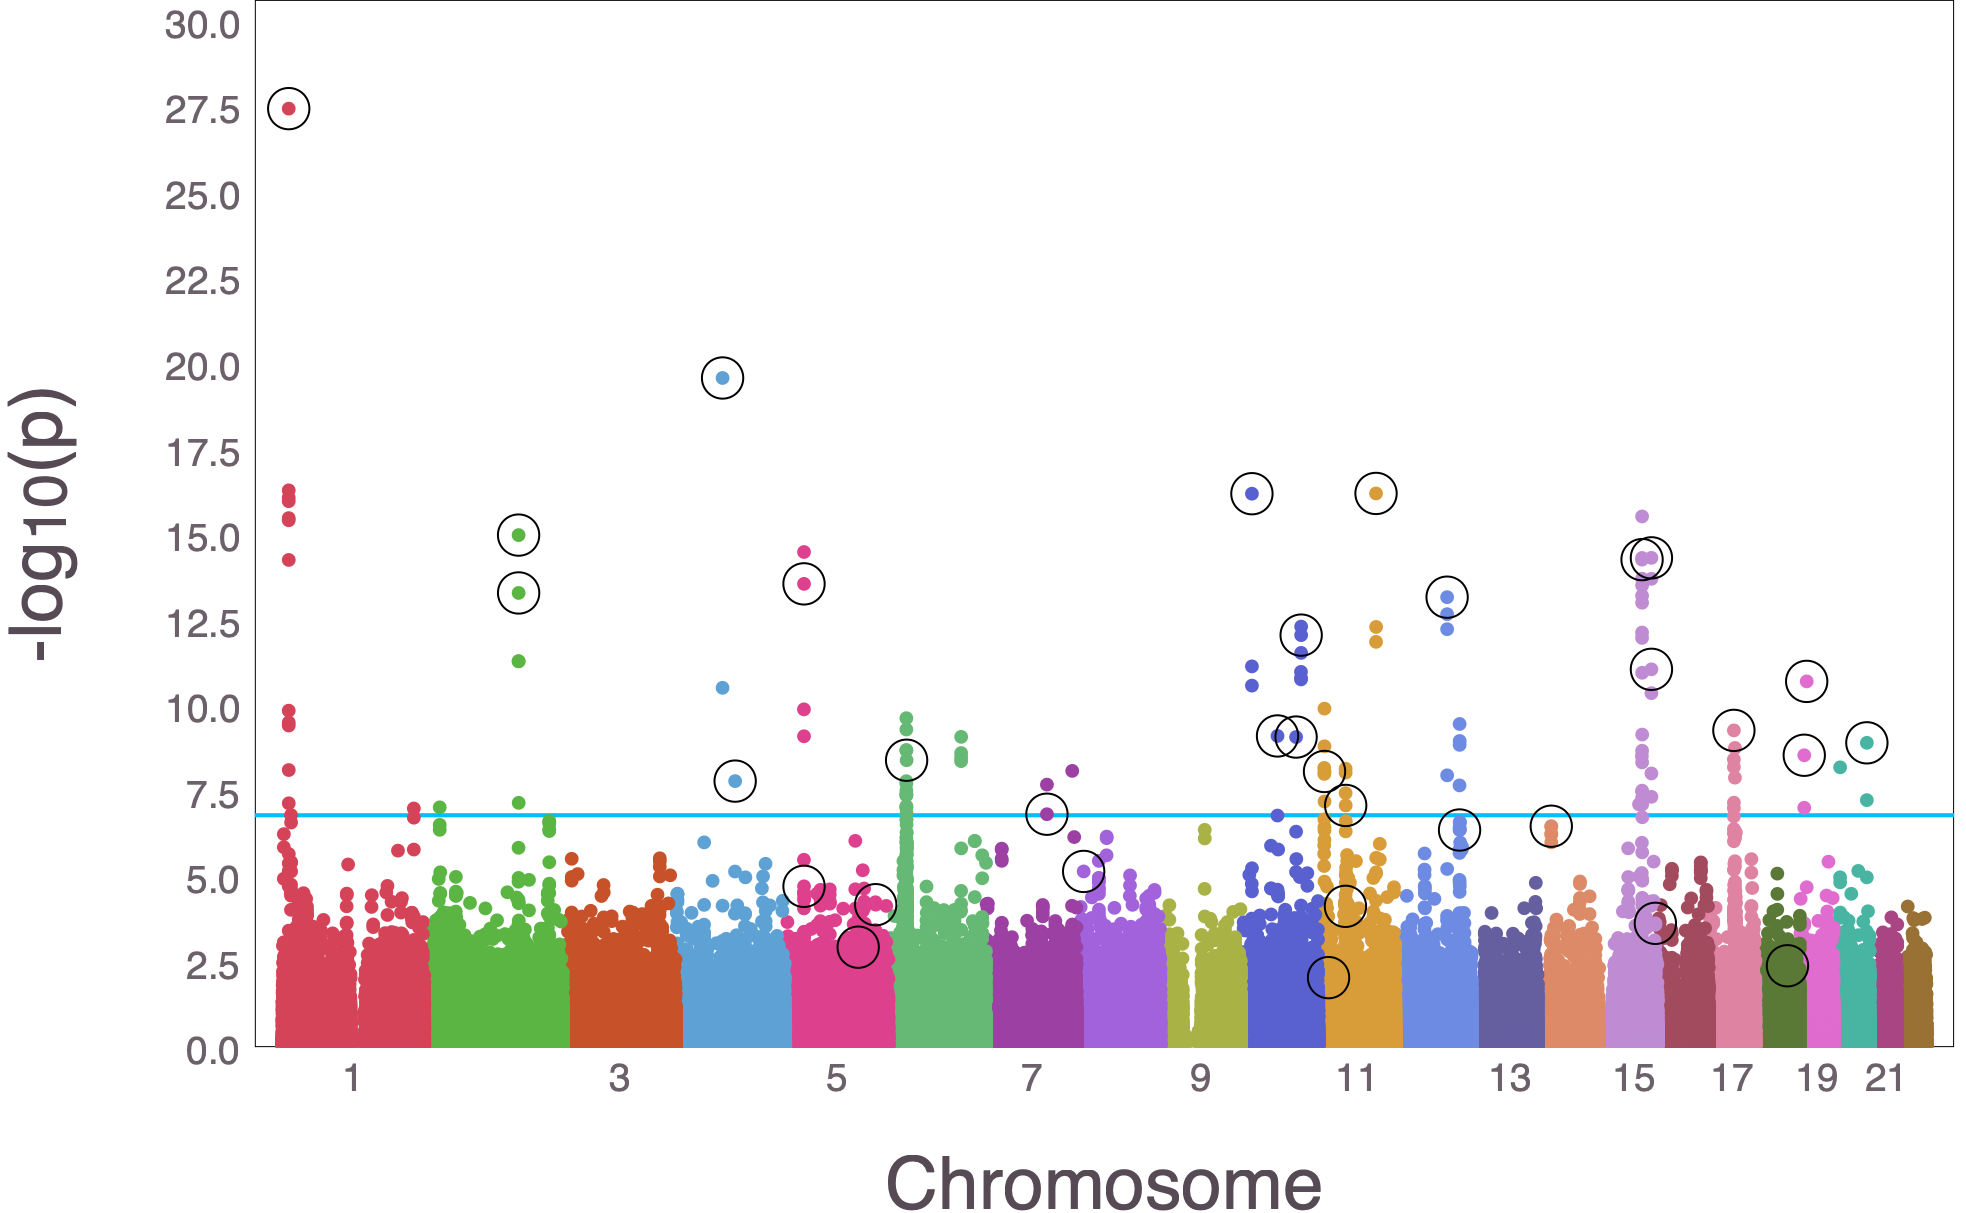
\includegraphics[width=\linewidth]{figures/manhattan_cropped.png}
    \caption{Manhattan plot comparing a logistic (univariate) GWAS vs logistic IHT on UK Biobank data ($n \approx 200,000$ and $p \approx 500,000$). Colored dots are $\log_{10}$ p-values from a logistic GWAS, and the circled dots are SNPs recovered by IHT.}
\end{figure}
}

\frame{
\frametitle{IHT related ongoing and potential future work}
\begin{enumerate}
    \item Multivariate Gaussian IHT - each sample measures $m$ (potentially correlated) phenotypes $\by_i^t = [y_{i1}, ..., y_{im}]$ \textbf{(ongoing)}
    \item Heritability estimates using IHT: since SNPs are estimated as mean effects, IHT will likely outperform mixed-model estimates whose SNPs are in the variance \textbf{(potential project)}
    \item Survival IHT - each sample $i$ has time-to-event measurement $y_i$ and indicator $I_i$ for event \textbf{(potential project)}
    \item Structured IHT - Each sample's phenotype $y_i$ take ordered, discrete values. \textbf{(potential project)}
    \item IHT vs transformed linear mixed model - Compare current IHT to mixed model approach where phenotypes are transformed to normal \textbf{(potential project)}
\end{enumerate}
}

\frame{
  \frametitle{Thank you!!}
  Visit us at: \url{https://github.com/OpenMendel/}
  \begin{figure}
      \centering \includegraphics[height=2.5in]{figures/openmendel.png}
      \caption{Weekly meetings from the OpenMendel group}
  \end{figure}
}

\frame{
\frametitle{References}
\begin{enumerate}
\item Chu, B. B., Keys, K. L., German, C. A., Zhou, H., Zhou, J. J., Sobel, E. M., ... \& Lange, K. (2020). Iterative hard thresholding in genome-wide association studies: Generalized linear models, prior weights, and double sparsity. {\it GigaScience}, 9(6), giaa044.
\item Chu, B. B., Sobel, E., Wasiolek, R., Sinsheimer, J. S., Zhou, H., \& Lange, K. (2020). A Fast Data-Driven Method for Genotyp Imputation, Phasing, and Local Ancestry Inference: MendelImpute. jl. {\it bioRxiv}.
\item Noah Zaitlen (2018)
A Short Tutorial on Linear Mixed Model Association Testing in Genetics.
\url{https://www.youtube.com/watch?v=pTAXVTA0YQQ}
\end{enumerate}
}

\end{document}
